\documentclass{article}
\usepackage[utf8]{inputenc}
\usepackage[T1]{fontenc}
\usepackage{graphicx} % do wstawiania wykresów
\usepackage{listings}
\usepackage{xcolor}
\lstset{
    language=C++,
    basicstyle=\ttfamily\small,
    keywordstyle=\color{blue},
    commentstyle=\color{gray},
    stringstyle=\color{orange},
    breaklines=true,
    frame=single,
    numbers=left,
    numberstyle=\tiny\color{gray},
    tabsize=4
}

% Autor i Data
\author{Jakub Gucwa}
\date{22 kwietnia 2026}

% Tytuł
\title{Optymalizacja Kodu na różne architektury: Zadanie 1}

\begin{document}

\maketitle

\section{Cel zadania}
Celem tego zadania jest zaimplementowanie funkcji przetwarzającej duże ciągi tekstowe. Funkcja powinna wykonywać następujące operacje:
\begin{itemize}
    \item Usuwanie znaków spoza zakresu drukowalnych.
    \item Zamiana sekwencji białych znaków na pojedynczą spację.
    \item Konwersja wszystkich liter na małe litery.
    \item Zamiana interpunkcji na przecinki.
    \item Eliminacja duplikatów wyrazów występujących jeden po drugim.
\end{itemize}

% Sekcje dla każdej wersji programu
\section{Wersja 1 - implementacja bazowa}
Wersja \texttt{normalize1.cpp} jest rozwiązaniem bazowym napisanym z użyciem klasy \texttt{std::string}. Algorytm przechodzi liniowo po całym wejściu i buduje nowy napis \texttt{result}. Dodatkowo utrzymywane są dwa bufory słów: \texttt{current\_word} (aktualnie czytane słowo) oraz \texttt{last\_word} (ostatnie zatwierdzone słowo), co pozwala usuwać duplikaty sąsiadujących wyrazów.

Kolejne etapy działania są następujące:
\begin{itemize}
    \item Dla każdego znaku sprawdzane jest, czy jest białym znakiem (\texttt{isspace}). Jeżeli tak, to sekwencja wielu białych znaków zostaje sprowadzona do pojedynczej spacji.
    \item Znaki spoza zakresu drukowalnego ASCII (mniejsze od 32 lub większe od 126) są pomijane.
    Ważne jest to, aby to był krok drugi, ponieważ niektóre białe znaki są spoza tego zakresu, a powinny być zamienione na spację.
    \item Znaki interpunkcyjne (\texttt{ispunct}) są zamieniane na przecinek.
    \item Każdy zachowany znak jest konwertowany do małej litery (\texttt{tolower}) i dopisywany do wyniku.
    \item Po zakończeniu słowa porównywane są \texttt{current\_word} i \texttt{last\_word}. Jeśli są identyczne, ostatnio dopisane słowo jest cofane z wyniku.
\end{itemize}
Na końcu wykonywana jest jeszcze kontrola dla ostatniego słowa (gdy wejście nie kończy się spacją). Złożoność czasowa jest liniowa względem długości tekstu, ale wersja tworzy wiele pomocniczych obiektów i często realokuje pamięć.
\begin{lstlisting}[caption={Kod funkcji \texttt{normalize\_string} w wersji 1}]
std::string normalize_string(std::string input){
    std::string result = "";
    std::string current_word = "";
    std::string last_word = "";
    unsigned int n = input.size(), i = 0;
    unsigned char ascii_val;
    while(i<n){
        ascii_val = (unsigned char)input[i];
        if(isspace(ascii_val)){
            if(!result.empty() && result.back() != ' '){
                if(!current_word.empty() && current_word == last_word){
                    result.resize(result.size() - current_word.size());
                } else {
                    result += ' ';
                }
                last_word = current_word;
                current_word = "";
            }
            i++; continue;
        }

        if(ascii_val < 32 || ascii_val >126){
            i++; continue;
        }
        if(ispunct(ascii_val)){
            ascii_val = ',';
        }
        current_word += tolower(ascii_val);
        result += tolower(ascii_val);
        i++;
        
    }
    if(!current_word.empty() && current_word == last_word){
            result.resize(result.size() - current_word.size());
        }
        
    return result;
}
\end{lstlisting}
\newpage
\section{Wersja 2 - optymalizacja zarządzania pamięcią}
Wersja \texttt{normalize2.cpp} zachowuje tę samą logikę normalizacji co wersja 1, ale optymalizuje zarządzanie pamięcią wyjścia. Najważniejsze zmiany:
\begin{itemize}
    \item Bufor wyniku jest od razu rezerwowany przez \texttt{result.resize(input.size())}, dzięki czemu zapis odbywa się przez indeks i ogranicza koszt wielokrotnego dopisywania.
    \item Wprowadzono licznik \texttt{result\_size}, który określa faktyczną długość danych w buforze i pozwala wykonywać operacje cofania bez kosztownych modyfikacji całego napisu.
    \item Dodano licznik \texttt{curr\_word\_size}, co upraszcza usuwanie zduplikowanego słowa przez jednorazowe zmniejszenie długości wyniku.
\end{itemize}
W porównaniu z wersją 1 zmniejsza to narzut alokacji i kopiowania, przy zachowaniu identycznego efektu końcowego.

\begin{lstlisting}[caption={Fragment optymalizacji funkcji \texttt{normalize\_string} w wersji 2}]
std::string result;
result.resize(input.size()); 
int result_size = 0;
// ...
result[result_size++] = tolower(ascii_val);
result_size -= curr_word_size;
// ...
// na koniec:
result.resize(result_size);
\end{lstlisting}
\newpage
\section{Wersja 3 - normalizacja in-place}
Wersja \texttt{normalize3.cpp} idzie dalej i wykonuje normalizację \textbf{in-place}, czyli bez tworzenia osobnego napisu wynikowego. Kluczowe zmiany względem wersji 2:
\begin{itemize}
    \item Funkcja przyjmuje referencję \texttt{std::string \&input} i modyfikuje ten sam bufor.
    \item Zastosowano dwa indeksy: \texttt{i} do odczytu oraz \texttt{j} do zapisu, co pozwala nadpisywać dane wejściowe wynikiem.
    \item Po zakończeniu przetwarzania wykonywane jest \texttt{input.resize(j)}, które odcina nieużywaną końcówkę.
\end{itemize}
Ta wersja redukuje zużycie pamięci i liczbę kopiowań, co zwykle poprawia wydajność dla dużych plików.

\begin{lstlisting}[caption={Kluczowe zmiany w funkcji \texttt{normalize\_string} w wersji 3}]
void normalize_string(std::string &input){
    unsigned int i = 0, j = 0;
    // ...
    if(j>0 && input[j-1] != ' '){
        if(!current_word.empty() && current_word == last_word){
            j -= curr_word_size;
        } else {
            input[j++] = ' ';
        }
    // ...
    input[j] = tolower(ascii_val);
    current_word += input[j];
    curr_word_size++;
    i++; j++;
    // ...
    input.resize(j); 
}
\end{lstlisting}
\newpage
\section{Wersja 4 - implementacja biblioteczna}
Wersja \texttt{normalize4.cpp} zmienia podejście implementacji - opiera się na algorytmach STL.
\begin{itemize}
    \item Wstępna transformacja wszystkich znaków realizowana jest przez \texttt{std::transform} (białe znaki na spację, interpunkcja na przecinek, litery na małe).
    \item Usuwanie znaków spoza zakresu drukowalnego wykonuje \texttt{std::remove\_if}.
    \item Redukcja wielu spacji do jednej realizowana jest przez \texttt{std::unique} z własnym predykatem.
    \item Usuwanie kolejnych duplikatów słów oparto o \texttt{std::string\_view}, \texttt{std::find} i \texttt{std::copy}.
\end{itemize}
W tej wersji znacznie bardziej widoczne są kolejne kroki, ale kosztem wiekszej liczby przebiegów po danych wejściowych, co sprawia, że dla bardzo dużych plików wersja ta jest wolniejsza od pozostałych.
\begin{lstlisting}[caption={Funkcja \texttt{normalize\_string} w wersji 4}]

void normalize_string(std::string &input){
    std::transform(input.begin(), input.end(),input.begin(),
        [](unsigned char c) -> char {
            if (isspace(c))  return ' ';
            if (ispunct(c))  return ',';
            return (char)tolower(c);
        });
    
    input.resize(
        std::remove_if(input.begin(), input.end(),
            [](unsigned char c){ return c < 32 || c > 126; })
        - input.begin());

    input.resize(
        std::unique(input.begin(), input.end(),
            [](char a, char b){ return a == ' ' && b == ' '; })
        - input.begin());

    auto word_begin = input.begin();
    auto write_end  = input.begin();
    std::string_view last_word;

    while (word_begin != input.end()) {
        auto word_end = std::find(word_begin, input.end(), ' ');
        std::string_view current(&*word_begin, (size_t)(word_end - word_begin));

        if (current != last_word) {
            if (write_end != input.begin()) *write_end++ = ' ';
            auto new_word_start = write_end;
            write_end = std::copy(word_begin, word_end, write_end);
            last_word = std::string_view(&*new_word_start, current.size());
        }

        word_begin = word_end;
        if (word_begin != input.end()) ++word_begin;
    }
    input.erase(write_end, input.end());
}
\end{lstlisting}
\section{Wersja 5 - optymalizacja z wykorzystaniem podstawowych tablic znaków}
Wersja \texttt{normalize5.cpp} przechodzi z C++-owych napisów na bufor \texttt{char*} i funkcje z biblioteki C. Algorytm jest oparty o ten z wersji 3, ale wprowadzono następujące zmiany:
\begin{itemize}
    \item Operacje wykonywane są na surowej tablicy znaków, co daje większą kontrolę nad pamięcią i ogranicza narzut abstrakcji \texttt{std::string}.
    \item Porównywanie słów do detekcji duplikatów wykorzystuje \texttt{memcmp}, a kopiowanie \texttt{memcpy}.
    \item Ostatnie słowo zapamiętywane jest w buforze \texttt{last\_word\_buf}, co pozwala szybko sprawdzić, czy bieżące słowo powtarza poprzednie.
\end{itemize}
Przez podejście niskopoziomowe algorytm jest szybszy, ale kod jest mniej czytelny.
\newpage
\begin{lstlisting}[caption={Kluczowy fragment funkcji \texttt{normalize\_string} w wersji 5}]
size_t normalize_string(char* p, size_t n){

    // ...
    char* last_word_buf = (char*)malloc(n + 1);

    while (i < n) {
        c = (unsigned char)p[i];

        if (isspace(c)) {
            if (j > 0 && p[j-1] != ' ') {
                if (curr_word_size > 0 && curr_word_size == last_word_len &&
                    memcmp(p + j - curr_word_size, last_word_buf, curr_word_size) == 0) {
                    j -= curr_word_size;
                } else {
                    memcpy(last_word_buf, p + j - curr_word_size, curr_word_size);
                    last_word_len = curr_word_size;
                    p[j++] = ' '; 
                }
                curr_word_size = 0;
            }
            i++;
            continue;
        }

        if (c < 32 || c > 126) { i++; continue; }
        if (ispunct(c)) c = ',';

        p[j++] = (char)tolower(c);
        curr_word_size++;
        i++;
    }
    // ...
    free(last_word_buf);
    p[j] = '\0';
    return j;
}

\end{lstlisting}
\newpage
\section{Wersja 6 - przetwarzanie wielowątkowe}
Wersja \texttt{normalize6.cpp} rozszerza wersję 5 o przetwarzanie wielowątkowe. Najważniejsze zmiany:
\begin{itemize}
    \item Wejście jest dzielone na fragmenty, a każdy fragment przetwarza osobny wątek (funkcja \texttt{partial\_normalize}).
    \item Granice fragmentów są przesuwane do granic słów (po białych znakach), aby nie zaczynać fragmentu w środku wyrazu.
    \item Po zakończeniu pracy wątków fragmenty są scalane do jednego bufora, z dodatkową obsługą duplikatów słów na granicach fragmentów.
\end{itemize}
W porównaniu z wersją 5 celem jest skrócenie czasu działania na dużych danych przez wykorzystanie wielu rdzeni procesora. Kosztem jest większa złożoność kodu i konieczność poprawnego scalenia wyników cząstkowych.

\begin{lstlisting}[caption={Podział na oddzielne zadania dla wątków w \texttt{normalize\_string} w wersji 6}]
for (size_t i = 1; i < num_threads; i++) {
    size_t pos = i * part_size;
    while (pos < n && !isspace((unsigned char)p[pos])) pos++;
    while (pos < n &&  isspace((unsigned char)p[pos])) pos++;
    frag_starts[i] = pos;  // granica na slowie
}
for (size_t i = 0; i < num_threads; i++) {
    size_t flen = frag_end - frag_starts[i];
    threads[i] = std::thread([=]() {
        frag_sizes[i] = partial_normalize(
            p + frag_starts[i], flen);
    });
}
for (size_t i = 0; i < num_threads; i++) threads[i].join();
\end{lstlisting}
\newpage
\section{Analiza profilera (gprof)}

Każdą implementację skompilowano z flagą \texttt{-pg} i uruchomiono 400-krotnie na pliku \texttt{regulartests/test1M}.
Wyniki zebrano narzędziem \texttt{gprof}.

\subsection*{Zestawienie wyników}

\begin{center}
\begin{tabular}{|c|l|r|r|r|}
\hline
\textbf{Wersja} & \textbf{Dominująca funkcja} & \textbf{\% czasu} & \textbf{Łączny czas} & \textbf{ms/call} \\
\hline
1 & \texttt{normalize\_string} (std::string)   & 91.9\% & 1.11 s & 2.55 \\
2 & \texttt{normalize\_string} (std::string)   & 91.3\% & 1.27 s & 2.90 \\
3 & \texttt{normalize\_string} (std::string\&) & 81.2\% & 1.17 s & 2.38 \\
4 & \texttt{normalize\_string} (std::string\&) & 93.2\% & 1.17 s & 2.73 \\
5 & \texttt{normalize\_string} (char*)         & 81.5\% & 0.81 s & 1.65 \\
6 & \texttt{partial\_normalize} (4 wątki)      & 80.9\% & 0.94 s & 0.475/wątek \\
\hline
\end{tabular}
\end{center}

\subsection*{Wnioski z profilowania}

\begin{itemize}
    \item We wszystkich wersjach praktycznie cały czas procesu spędza się wewnątrz funkcji normalizującej (80--93\%), co potwierdza, że główne wąskie gardło leży w logice przetwarzania znaków, nie w I/O ani inicjalizacji.
    \item \textbf{Wersja 1 vs 2}: Wersja 2 wykazała nieco wyższy czas z profilerem (1.27 s vs 1.11 s) -- narzut instrumentacji \texttt{-pg} zaburza pomiar przy dużej liczbie małych operacji na \texttt{std::string}.
    \item \textbf{Wersja 3}: Operacja in-place (bez tworzenia osobnego bufora) obniżyła ms/call do 2.38 -- mniej alokacji pamięci przekłada się na realną poprawę.
    \item \textbf{Wersja 4}: Podejście STL (kilka przebiegów \texttt{transform}/\texttt{remove\_if}/\texttt{unique}) okazało się wolniejsze od wersji 3 (2.73 ms/call) -- kolejne przebiegi po danych generują dodatkowy narzut cache.
    \item \textbf{Wersja 5}: Przejście na surowy bufor \texttt{char*} z \texttt{memcmp}/\texttt{memcpy} przyniosło największą poprawę spośród implementacji jednowątkowych (1.65 ms/call, łączny czas 0.81 s).
    \item \textbf{Wersja 6}: Wielowątkowość (4 wątki) skróciła realny czas wykonania do 0.355 s (pomiar bez \texttt{-pg}). Gprof mierzy 80.9\% czasu w \texttt{partial\_normalize} wywoływanym 1600 razy (400 iter. $\times$ 4 wątki). Łączny czas gprof (0.94 s) jest sumą czasu wszystkich wątków, nie rzeczywistego czasu wykonania, z czego pozorne spowolnienie względem wersji 5 w tabeli powyżej.
\end{itemize}
\newpage
\section{Analiza profilera (perf)}

Dla każdej wersji wykonano pomiar \texttt{perf} (\texttt{record -e cycles:u -F 999}) na danych \texttt{regulartests/test1M}. Poniżej zestawiono czas pojedynczego uruchomienia programu oraz główny hotspot z raportu \texttt{perf report}.

\begin{center}
\begin{tabular}{|c|r|r|l|}
\hline
\textbf{Wersja} & \textbf{Czas [s]} & \textbf{Top \% (perf)} & \textbf{Najgorętszy symbol} \\
\hline
1 & 1.562987 & 73.18\% & \texttt{normalize\_string(std::string)} \\
2 & 1.586685 & 70.17\% & \texttt{normalize\_string(std::string)} \\
3 & 1.442242 & 70.12\% & \texttt{normalize\_string(std::string\&)} \\
4 & 1.196079 & 82.10\% & \texttt{normalize\_string(std::string\&)} \\
5 & 0.966707 & 70.45\% & \texttt{normalize\_string(char*, size\_t)} \\
6 & 0.311479 & 88.89\% & \texttt{normalize\_string}/\texttt{partial\_normalize} \\
\hline
\end{tabular}
\end{center}

\subsection*{Wnioski z perf}
\begin{itemize}
    \item We wszystkich implementacjach główny koszt CPU pozostaje w funkcji normalizującej; udział funkcji wynosi około 70--82\% (dla wersji 1--5).
    \item Dla wersji 1--5 drugim wyraźnym kosztem jest \texttt{\_\_ctype\_tolower\_loc@plt}, co jest niczym niespodziewanym, ponieważ każdy zapisywany znak wywołuje \texttt{tolower}.
    \item Wersja 6 ma najniższy czas ściany (0.311 s).
\end{itemize}

% Sekcja na wykresy
\section{Wykresy}

\begin{figure}[h!]
    \centering
    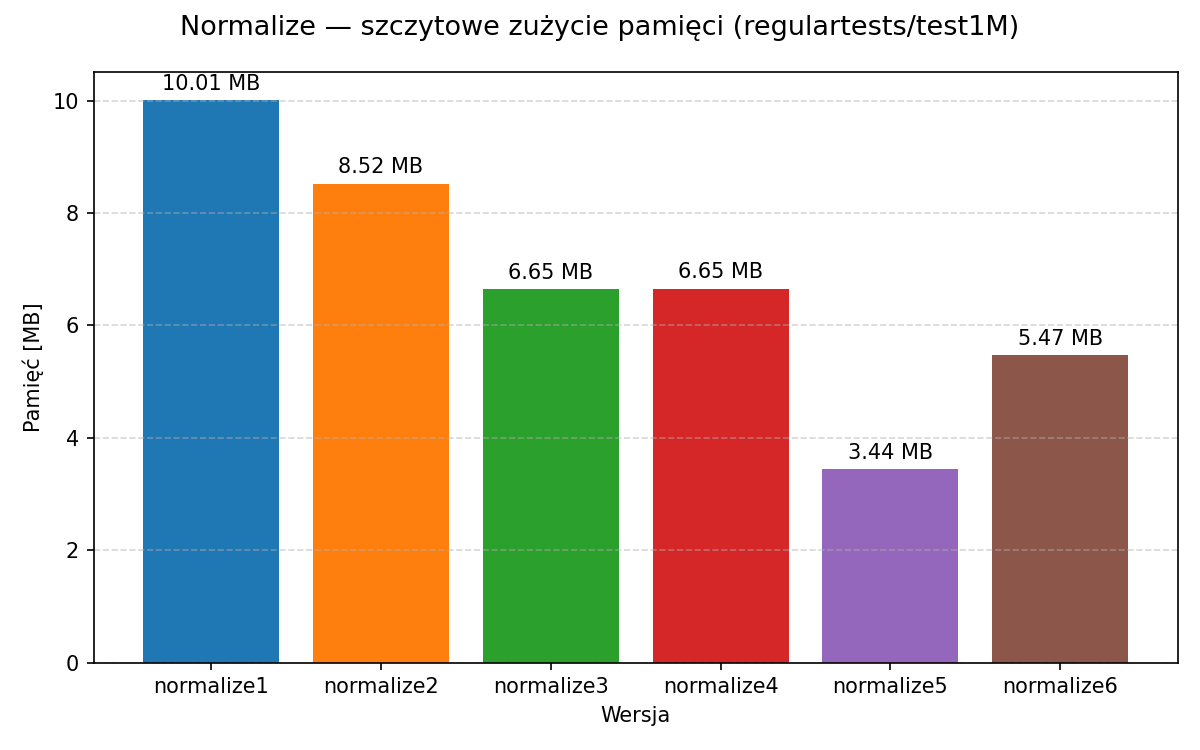
\includegraphics[width=0.8\textwidth]{chart_memory.png}
    \caption{Wykres użycia pamięci.}
    \label{fig:memory}
\end{figure}

\begin{figure}[h!]
    \centering
    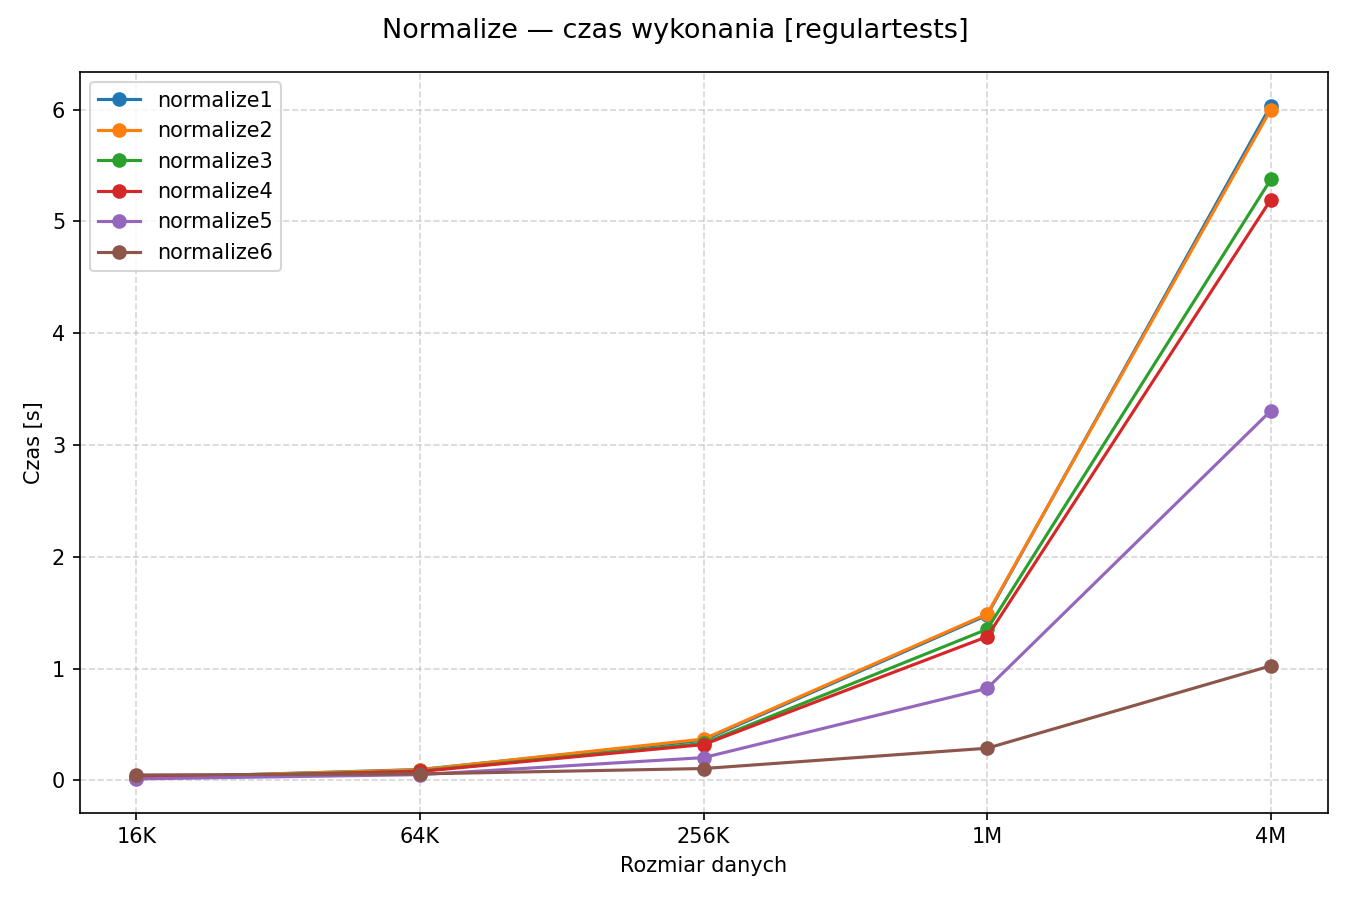
\includegraphics[width=0.8\textwidth]{chart_regulartests.png}
    \caption{Czas działania poszczególnych implementacji -- dane regularne.}
    \label{fig:regulartests}
\end{figure}

\begin{figure}[h!]
    \centering
    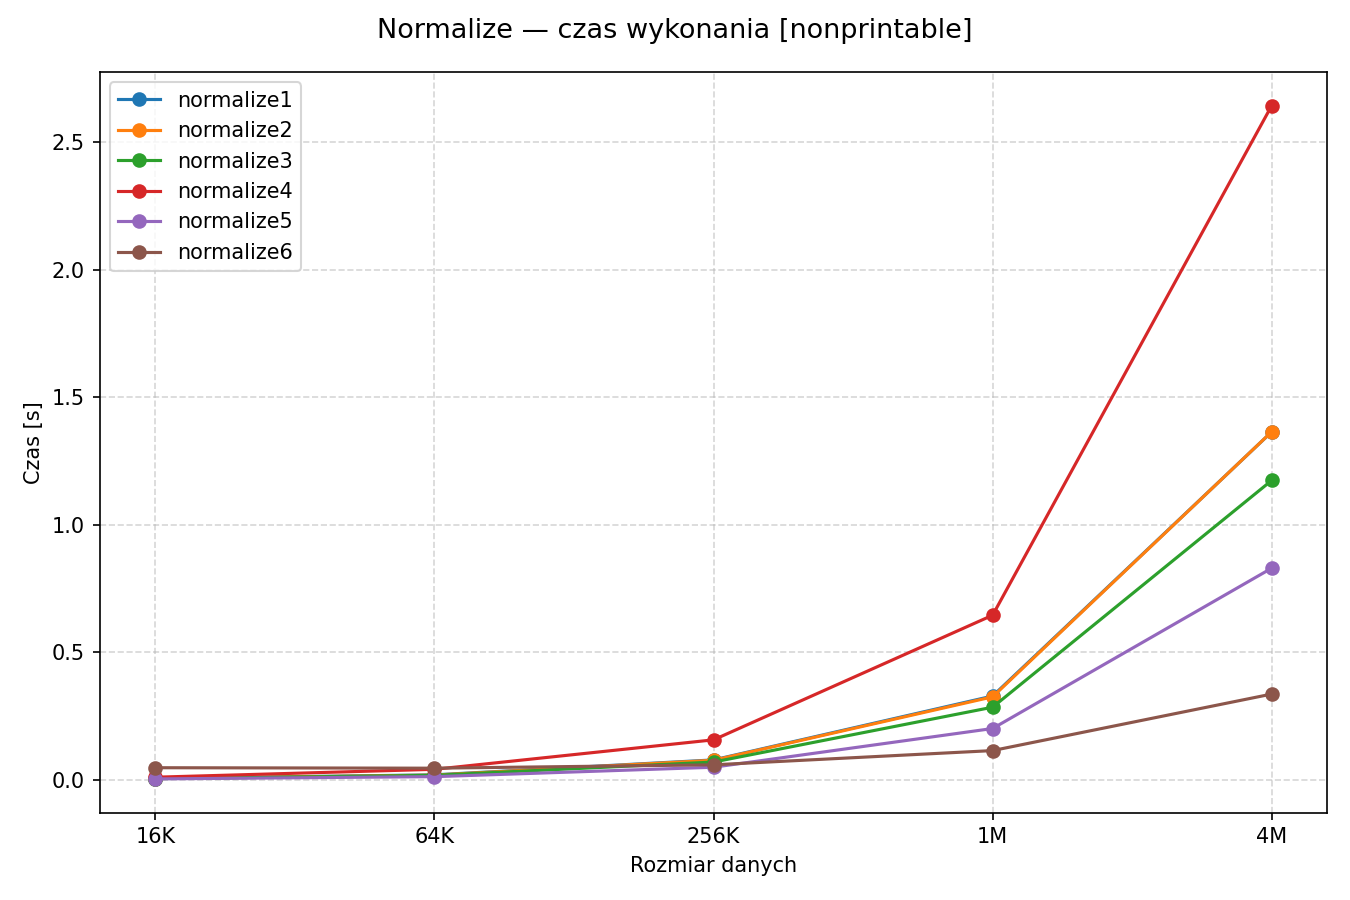
\includegraphics[width=0.8\textwidth]{chart_nonprintable.png}
    \caption{Czas działania poszczególnych implementacji -- głównie niedrukowalne znaki.}
    \label{fig:nonprintable}
\end{figure}

\begin{figure}[h!]
    \centering
    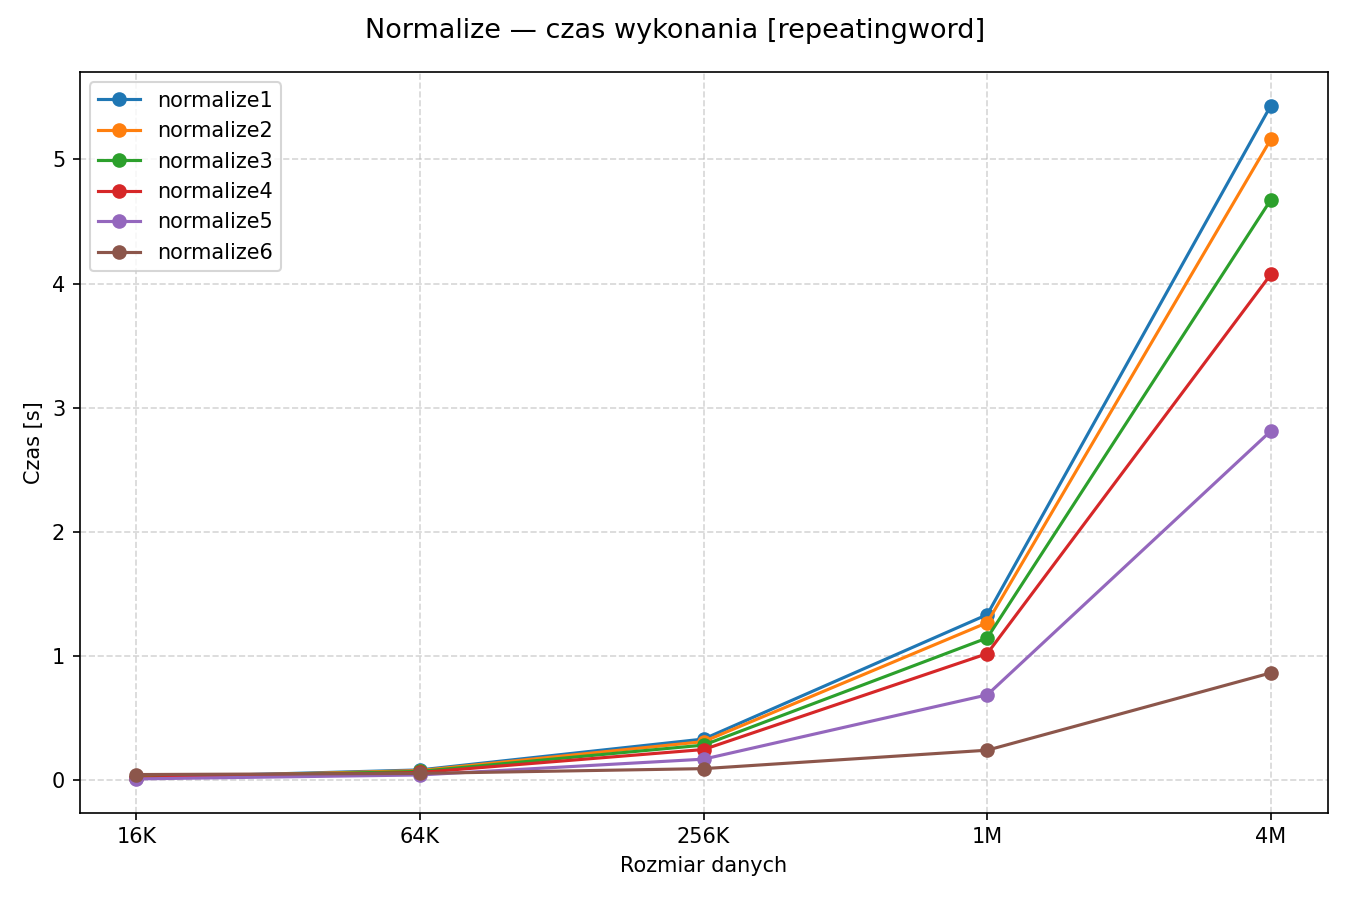
\includegraphics[width=0.8\textwidth]{chart_repeatingword.png}
    \caption{Czas działania poszczególnych implementacji -- głównie powtarzające się wyrazy.}
    \label{fig:repeatingword}
\end{figure}

\begin{figure}[h!]
    \centering
    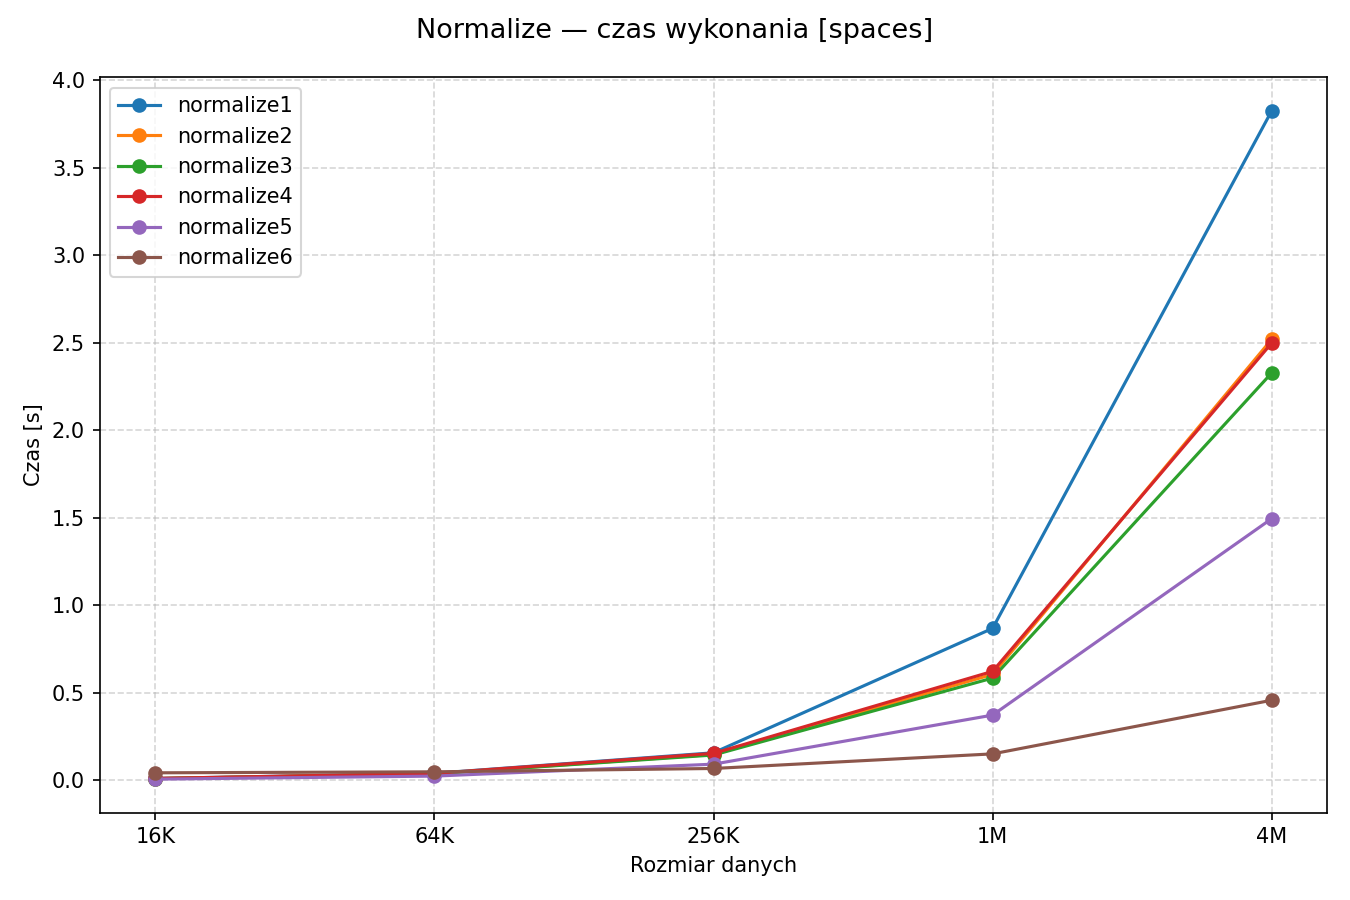
\includegraphics[width=0.8\textwidth]{chart_spaces.png}
    \caption{Czas działania poszczególnych implementacji -- głównie białe znaki.}
    \label{fig:spaces}
\end{figure}

\end{document}